\chapter{Metodologia}

\section{Objetivos}

O objetivo deste capítulo é apresentar a metodologia utilizada para a
realização da pesquisa e contribuição tecnológica. A principal questão
a ser respondida é: como a visualização de software pode auxiliar na
interpretação das métricas coletas e calculadas por ferramentas de análise
de código?

Considerando esta questão, é importante ressaltar que existem incontáveis
destas ferramentas. Porém estas analisam apenas aspectos mui específicos
do software, e falham (algumas delas) em demostrar ao engenheiro de
qualidade a interpretação dos dados analisados \cite{deissenboeck2011}.

Neste trabalho serão unidas determinadas métricas (TODO: definir quais
métricas), para gerar uma ou várias visualizações que auxiliem o usuário
do Mezuro a ter uma melhor interpretação do resultado gerado por esta
ferramenta.

Como exemplo dessa união e para a construção da prova de conceito
(TODO: é esse mesmo o nome?), é proposto utilizar-se da decisão dos
colegas Renan Costa Filgueiras e Vinícius Vieira Meneses: foram escolhidas
três métricas para a configuração da visualização em radar: \textit{number
of methods} (código: npm), \textit{number of public methods} (código nom)
e \textit{total number of modules} (código: total\_modules); e a decisão
de utilizar a biblioteca Javascript \textit{D3.js - Data-Driven Documents}.
(TODO: adicionar referência)

\section{Trabalhos Relacionados}

\section{Questão Problema e Hipóteses}

Reforçando a questão problema (QP), foram levantadas estas outras abaixo:

\begin{itemize}
  \item QP1 - Como a visualização de software pode auxiliar na
  interpretação das métricas coletadas e calculadas pelo Mezuro?
  \item QP2 - Quais técnicas de visualização que melhor se adequam ao
  contexto do Mezuro, possibilitando a aplicação em qualquer contexto de
  configuração?
  \item QP3 - Como representar as diferentes perspectivas sobre o processo
  de desenvolvimento e o produto de software?
\end{itemize}

As hipóteses são:

\begin{itemize}
  \item H1 - Não haverá uma visualização única para todas as métricas.
  \item H2 - Algumas métricas poderão ser apresentadas de uma forma combinada
  em uma única represetação/visualização.
\end{itemize}

% TODO: elaborar e documentar as hipótees

\section{O Mezuro}

O projeto Mezuro é uma ferramenta para extração, análise e interpretação de
métricas de código-fonte. De uma forma geral, ele é dividido em duas partes:
para o processamento e para o cálculo é utilizado o Kalibro, que é um
\textit{webservice}; e o Prezento para a interface gráfica (uma aplicação
\textit{Web}) \cite{meirellesCibse2015}. Sob a licença
\textit{Affero General Public License version 3} (AGPLv3), o Mezuro permite que
o usuário crie, salve e edite ``configurações'' que são um conjunto de
métricas escolhidas por este e um ``grupo de leitura'' para provimento de uma
interface gráfica de um conjunto de leitura que tenha algum sentido quando
agrupadas, por exemplo: com a pontuação x, a métrica terá o ``rótulo'' ``BOM'' e
será atribuído à ela a cor amarela; com a pontuação x+2, a métrica terá o 
``rótulo'' ``ÓTIMO'' e estará com a cor verde. As cores são para destacar a
interpretação e são definidas com valores hexadecimal \cite{camarinhaOSS2015}.

O Kalibro, citado no parágrafo anterior, foi inicialmente escrito em Java para
compor uma das ferramentas do projeto QualiPSo (\textit{Quality Platform for
Open Source Software}). Já possuía maioria das funcionalidades presentes na
versão atual do Mezuro. Uma delas, bastante prática, é a de fornecer apenas o
URL do código compactado em arquivo ZIP ou TARBALL, ou o link para as
aplicações de controle de versão em SVN ou GIT, mais a escolha de uma
configuração, para iniciar a análise \cite{camarinhaOSS2015}. Em 2013 o Mezuro
passou a ser reescrito em Ruby, com objetivo de manter na mesma tecnologia as
camadas da arquitetura. Mudança justificada também pela necessidade do
processamento dos cálculos e da análise. A carga de requisições, mais a
quantidade de núcleos que o servidor possuía, faziam com que a versão original
do Kalibro ficasse debilitado em seu fluxo de execuções. Outra vantagem dessa
reescrita é a facilidade com que novos contribuidores puderam/poderão entender
todo o funcionamento dessa parte do Mezuro. Algumas funcionalidades foram
eliminadas por serem consideradas não essenciais. E grande parte da primeira
versão do Kalibro está presente na gema
kalibro\_gem\footnote{\url{https://rubygems.org/gems/kalibro_gem}}
\cite{meirellesCibse2015}.

% TODO: a gem kalibro\_gem e a kalibro\_client são a mesma coisa? A kalibro\_gem
% foi descontinuada?)

% Sobre o Prezento

O Kalibro foi construído, nos primórdios, como um plugin da rede social
Noosfero. Com a decisão de reescrevê-lo em Ruby, a antiga interface gráfica,
que era aproveitada do Noosfero, foi também reescrita nesta
tecnologia. O Prezento, desenvolvido utilizando o \textit{framework} para
desenvolvimento de aplicações \textit{Web}
Ruby on Rails\footnote{\url{http://guides.rubyonrails.org/getting_started.html}},
é a redesenha e atual interface.

% Sobre a arquitetura do Mezuro

% (Eu preciso falar do QualiPSo?  Não!)

O projeto QualiPSo, iniciado em meados de 2007, tinha como objetivo aprimorar
as práticas de desenvolvimento aberto à época para atingir o reconhecimento e
confiabilidade que o FOSS possui hoje \cite{messias2012}.

\subsection{Arquitetura e principais funcionalidades do Mezuro}

Com a reescrita, a arquitetura do Mezuro foi dividida em três serviços:

\begin{itemize}
  \item Prezento: para a interface gráfica do usuário
  \item Kalibro Processor: para a análise do código
  \item Kalibro Configuratios: para o gerenciamento das configurações
\end{itemize}

A decisão de dividir o Kalibro em serviços separados foi tomada para deixar
cada um deles com menos responsabilidades, facilitando a manutenção e evolução
\cite{camarinhaOSS2015}. E a comunicação entre estes serviços é feita através
do Kalibro Client: um quarto software também escrito em Ruby, mantendo a
escolha de centralização em uma única tecnologia. E para simplificar a
implementação, também foi decidido que a comunicação entre os serviços seria
RESTful.

As figuras a seguir demonstram como a comunicação funciona, um diagrama UML de
sequência do processo de criação de uma configuração chegando ao estágio em que
são expostos os resultados finais de uma análise após a reescrita da interface
gráfica, e outra que demonstra o estado atual do projeto.

% TODO: Alterar essa primeira imagem para representação da atual arquitetura

\begin{figure}[!htb]
	\centering
	\label{mezuroNoosferoArch}
		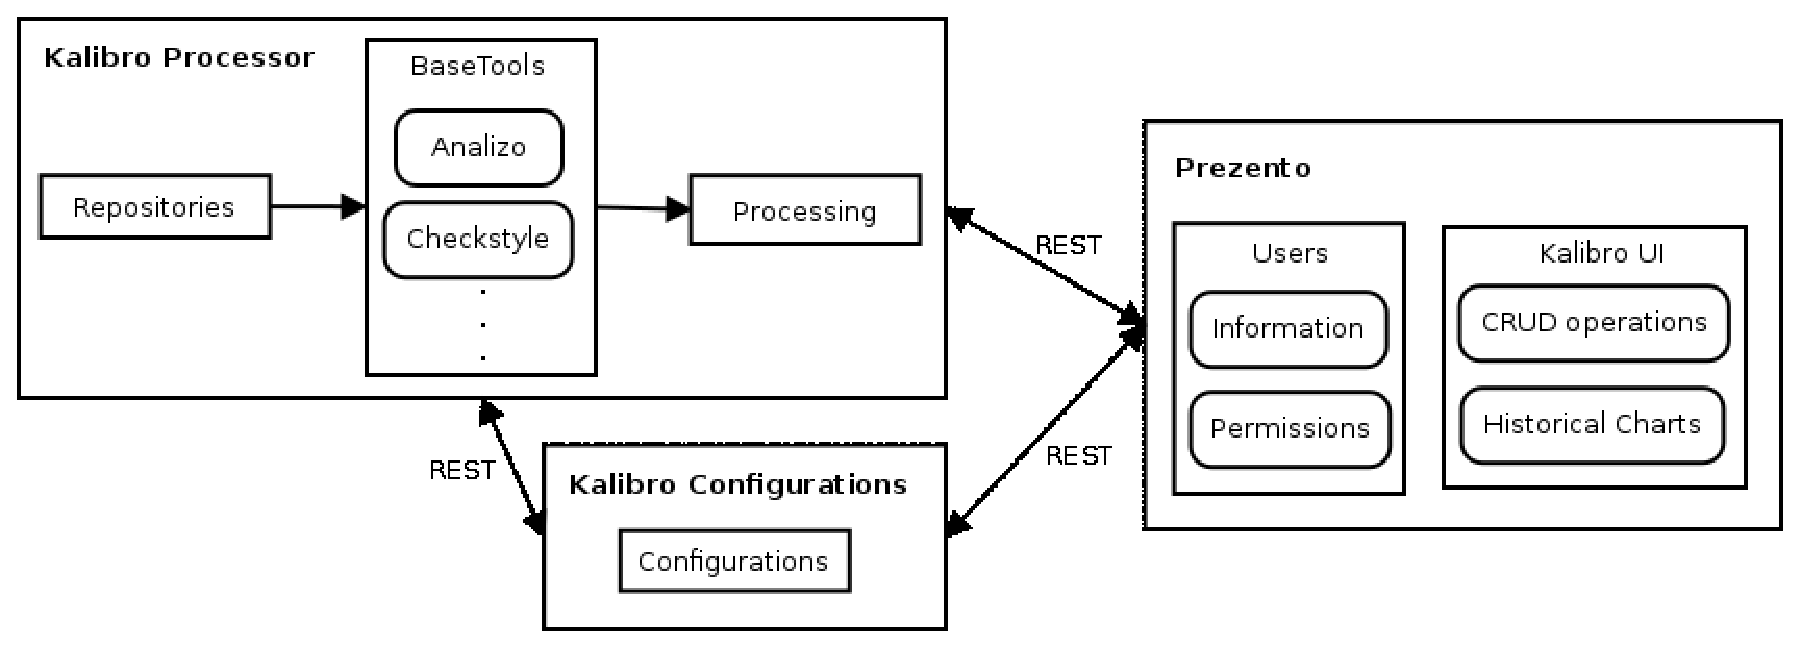
\includegraphics[keepaspectratio=true,scale=0.5]{figuras/mezuroCloudArch.eps}
	\caption{Arquitetura do Mezuro \cite{camarinhaOSS2015}}
\end{figure}

\begin{figure}[!htb]
	\centering
	\label{prevProcessingSeqDiag}
		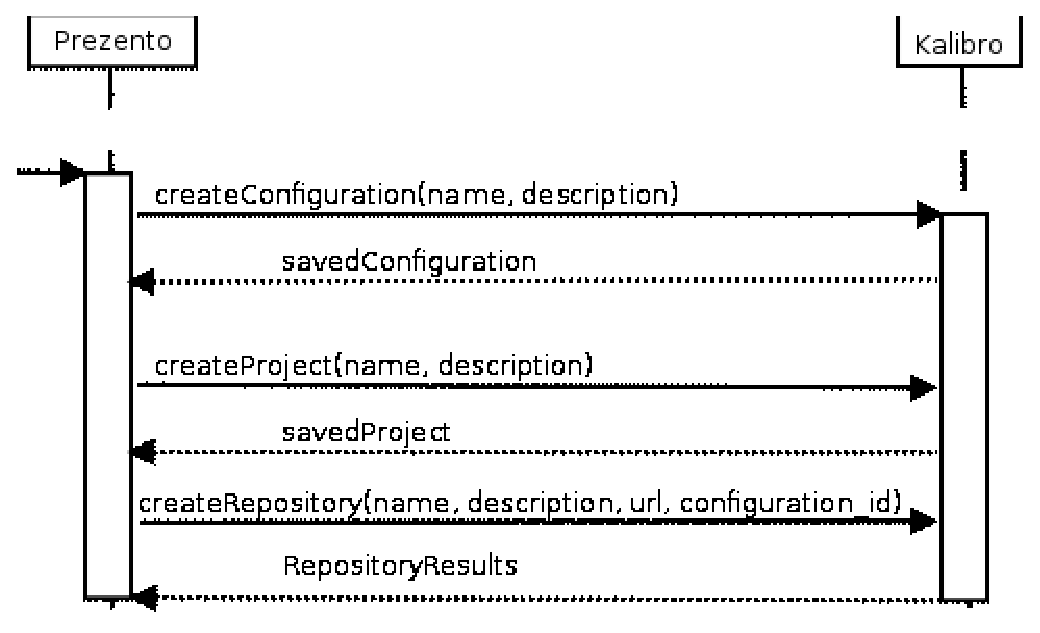
\includegraphics[keepaspectratio=true,scale=0.7]{figuras/prevProcessingSeqDiag.eps}
	\caption{Arquitetura do sistema ao fim da reescrita da interface gráfica
	\cite{meirellesCibse2015}}
\end{figure}

\begin{figure}[!htb]
	\centering
	\label{processingSeqDiag}
		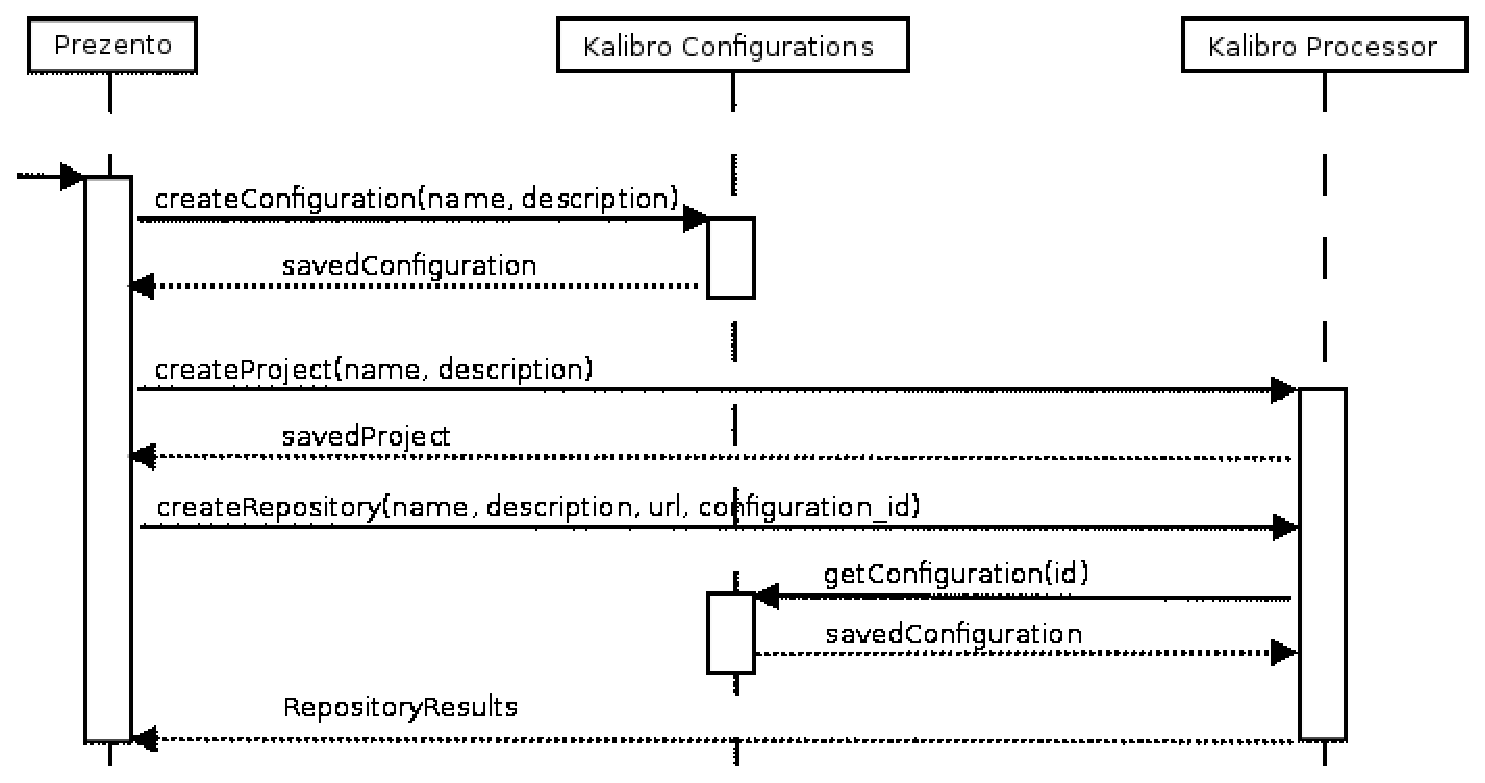
\includegraphics[keepaspectratio=true,scale=0.5]{figuras/processingSeqDiag.eps}
	\caption{Arquitetura do sistema ao fim da reestruturação do Kalibro
	\cite{meirellesCibse2015}}
\end{figure}

\newpage

Segundo \citeonline{camarinhaOSS2015}, as principais ``funcionalidades podem ser
divididas em dois grupos:

\begin{itemize}
  \item Projeto
    \begin{itemize}
    \item \textit{Download} do código-fonte a partir de repositórios (Git,
    Subversion, Bazaar etc) ou via arquivo compactado;
        \item Escolha da periodicidade do processamento do código (1 dia, 2 dias,
        semanal, quinzenal e mensal);
        \item Escolha de qual configuração de métricas cada repositório irá
        utilizar;
        \item Nota de cada métrica da configuração para cada arquivo do
        repositório;
        \item Análise gráfica de cada arquivo do repositório por meio de um
        gráfico de pontos com notas ao longo do tempo;
        \item Resultados públicos e acessíveis à comunidade.
    \end{itemize}
    \item Configuração
    \begin{itemize}
    \item Criação de configuração e a possibilidade de clonagem;
        \item Estatísticas sobre as configurações mais populares dentro da
        comunidade;
        \item Criação de intervalos qualitativos associados aos valores das
        métricas;
        \item Criação de grupos de leitura para a interpretação textual dos
        resultados das métricas;
        \item Combinações de métricas nativas para criação de análises compostas
        e mais complexas.''
    \end{itemize}
\end{itemize}
''
% TODO: consertar estas aspas na citação direta
% TODO: posso fazer esta citação direta?

\newpage

\section{A Decisão de utilizar o Mezruo}

Para este trabalho de conclusão de curso a ferramenta de de análise de código
fonte escolhida foi o Mezuro pois: o aluno já participou da evolução de parte
de algumas funcionalidades; a ferramenta proporciona ao usuário a análise
periódica do projeto, o que atende ao desejado como contribuição tecnológica
das visualizações geradas serem demonstradas ao longo do tempo; por ser uma
plataforma livre; fácil contato com os mantenedores; e por esta plataforma
estar sempre utilizar as últimas versões estáveis do Ruby e do Rails, ou seja,
por utilizar o que há de mais atual nestas tecnologias.

% TODO: deve adicionar mais motivações? Quais? Sei que devo, porém estou sem ideias

É importante ressaltar que outras ferramentas de análise de código poderão ser
utilizadas para geração da visualização proposta neste trabalho. Pois o fluxo
básico de execução permitirá tal geração, a saber: análise pela ferramenta,
dados exportados de forma determinada para anteder a leitura da biblioteca JS,
geração da visualização em um terceiro serviço local ou remoto.

E o ideal é que este trabalho sirva como base para a criação de futuras
visualizações para o Mezuro em si.

\section{Proposta de Evolução da Visualização}

\section{Seleção das Métricas}

% TODO: selecionar métricas com certo nível de similaridade.
% TODO: citar aqui talvez Michelle Lanza e R Marinescu - software metrics
